
\maketitle% this prints the handout title, author, and date

\begin{abstract}
\noindent
In performing this experiment, students should learn how to apply a variety of techniques to analyzing a chemical system. By using cytochrome \emph{c} as a model system, students will learn how to determine the free energy associated with unfolding a protein. Students will also learn the principles of fluorescence quenching via Förster energy transfer and then they will calculate intramolecular distances for partially unfolded and fully folded protein structures.\thanks{Transcribed and adapted from \textcite{sanchez08}.}
\end{abstract}

\section{Introduction} % (fold)

The study of biological macromolecular structure has become a major field in biochemistry and chemistry research laboratories. 
Numerous spectroscopic techniques, such as UV-Vis absorption, fluorescence, and circular dichroism, have been employed to investigate the thermodynamics and structural changes associated with protein folding and unfolding. 
In undergraduate laboratories, most experiments rely on a single technique to study a chemical problem. 
In this lab, a multifaceted approach is used to the study of the important biophysical problem of protein folding. 
Specifically, the combination of absorption, fluorescence, and Förster resonance energy transfer (FRET) techniques will provide complementary and in-depth information on structural changes and thermodynamics associated with these changes. 
The protein used in this experiment is a well-studied system, cytochrome \emph{c} (cyt \emph{c}). 
Cyt \emph{c} will be unfolded chemically via a denaturant and monitored spectroscopically. 

FRET is a spectroscopic technique that may be used to determine inter- or intramolecular distances. 
It has been applied to study a wide variety of systems to obtain structural information. 
FRET occurs via long-range dipole-dipole interactions between donor and acceptor molecules, and does not involve emission of a photon. 
Radiationless energy transfer from an excited-state donor to a ground-state acceptor is the fundamental principle behind FRET\@. 
A critical requirement for FRET is spectral overlap between the emission spectrum of the donor and the absorption spectrum of the acceptor. 
The efficiency of FRET energy transfer is inversely proportional to the sixth power of the distance between the donor and acceptor. 
By utilizing this distance dependence, structural information about proteins can be obtained during denaturant-induced unfolding. 

Cyt \emph{c} is an electron transfer protein found in the inner membrane of mitochondria. 
This globular protein consists of a single polypeptide chain that contains one tryptophan residue at position 59 (Trp-59) and a covalently bound heme cofactor. 
The intrinsic fluorophore, tryptophan, serves as the FRET donor while the heme cofactor serves as the acceptor. 
In the native structure of cyt \emph{c}, Trp-59 is in close proximity to the heme group (\cref{fig:cyt_c}). 
When the protein is folded, energy is transferred from the excited tryptophan to the heme group, causing the tryptophan fluorescence to be quenched. 
Upon addition of a chemical denaturant to unfold the protein, the rise in fluorescence signal from Trp-59 indicates that the distance between donor and acceptor has increased; this change in distance as a function of folding state can be quantified via the equations that describe FRET\@.
\begin{marginfigure}
	\centering
		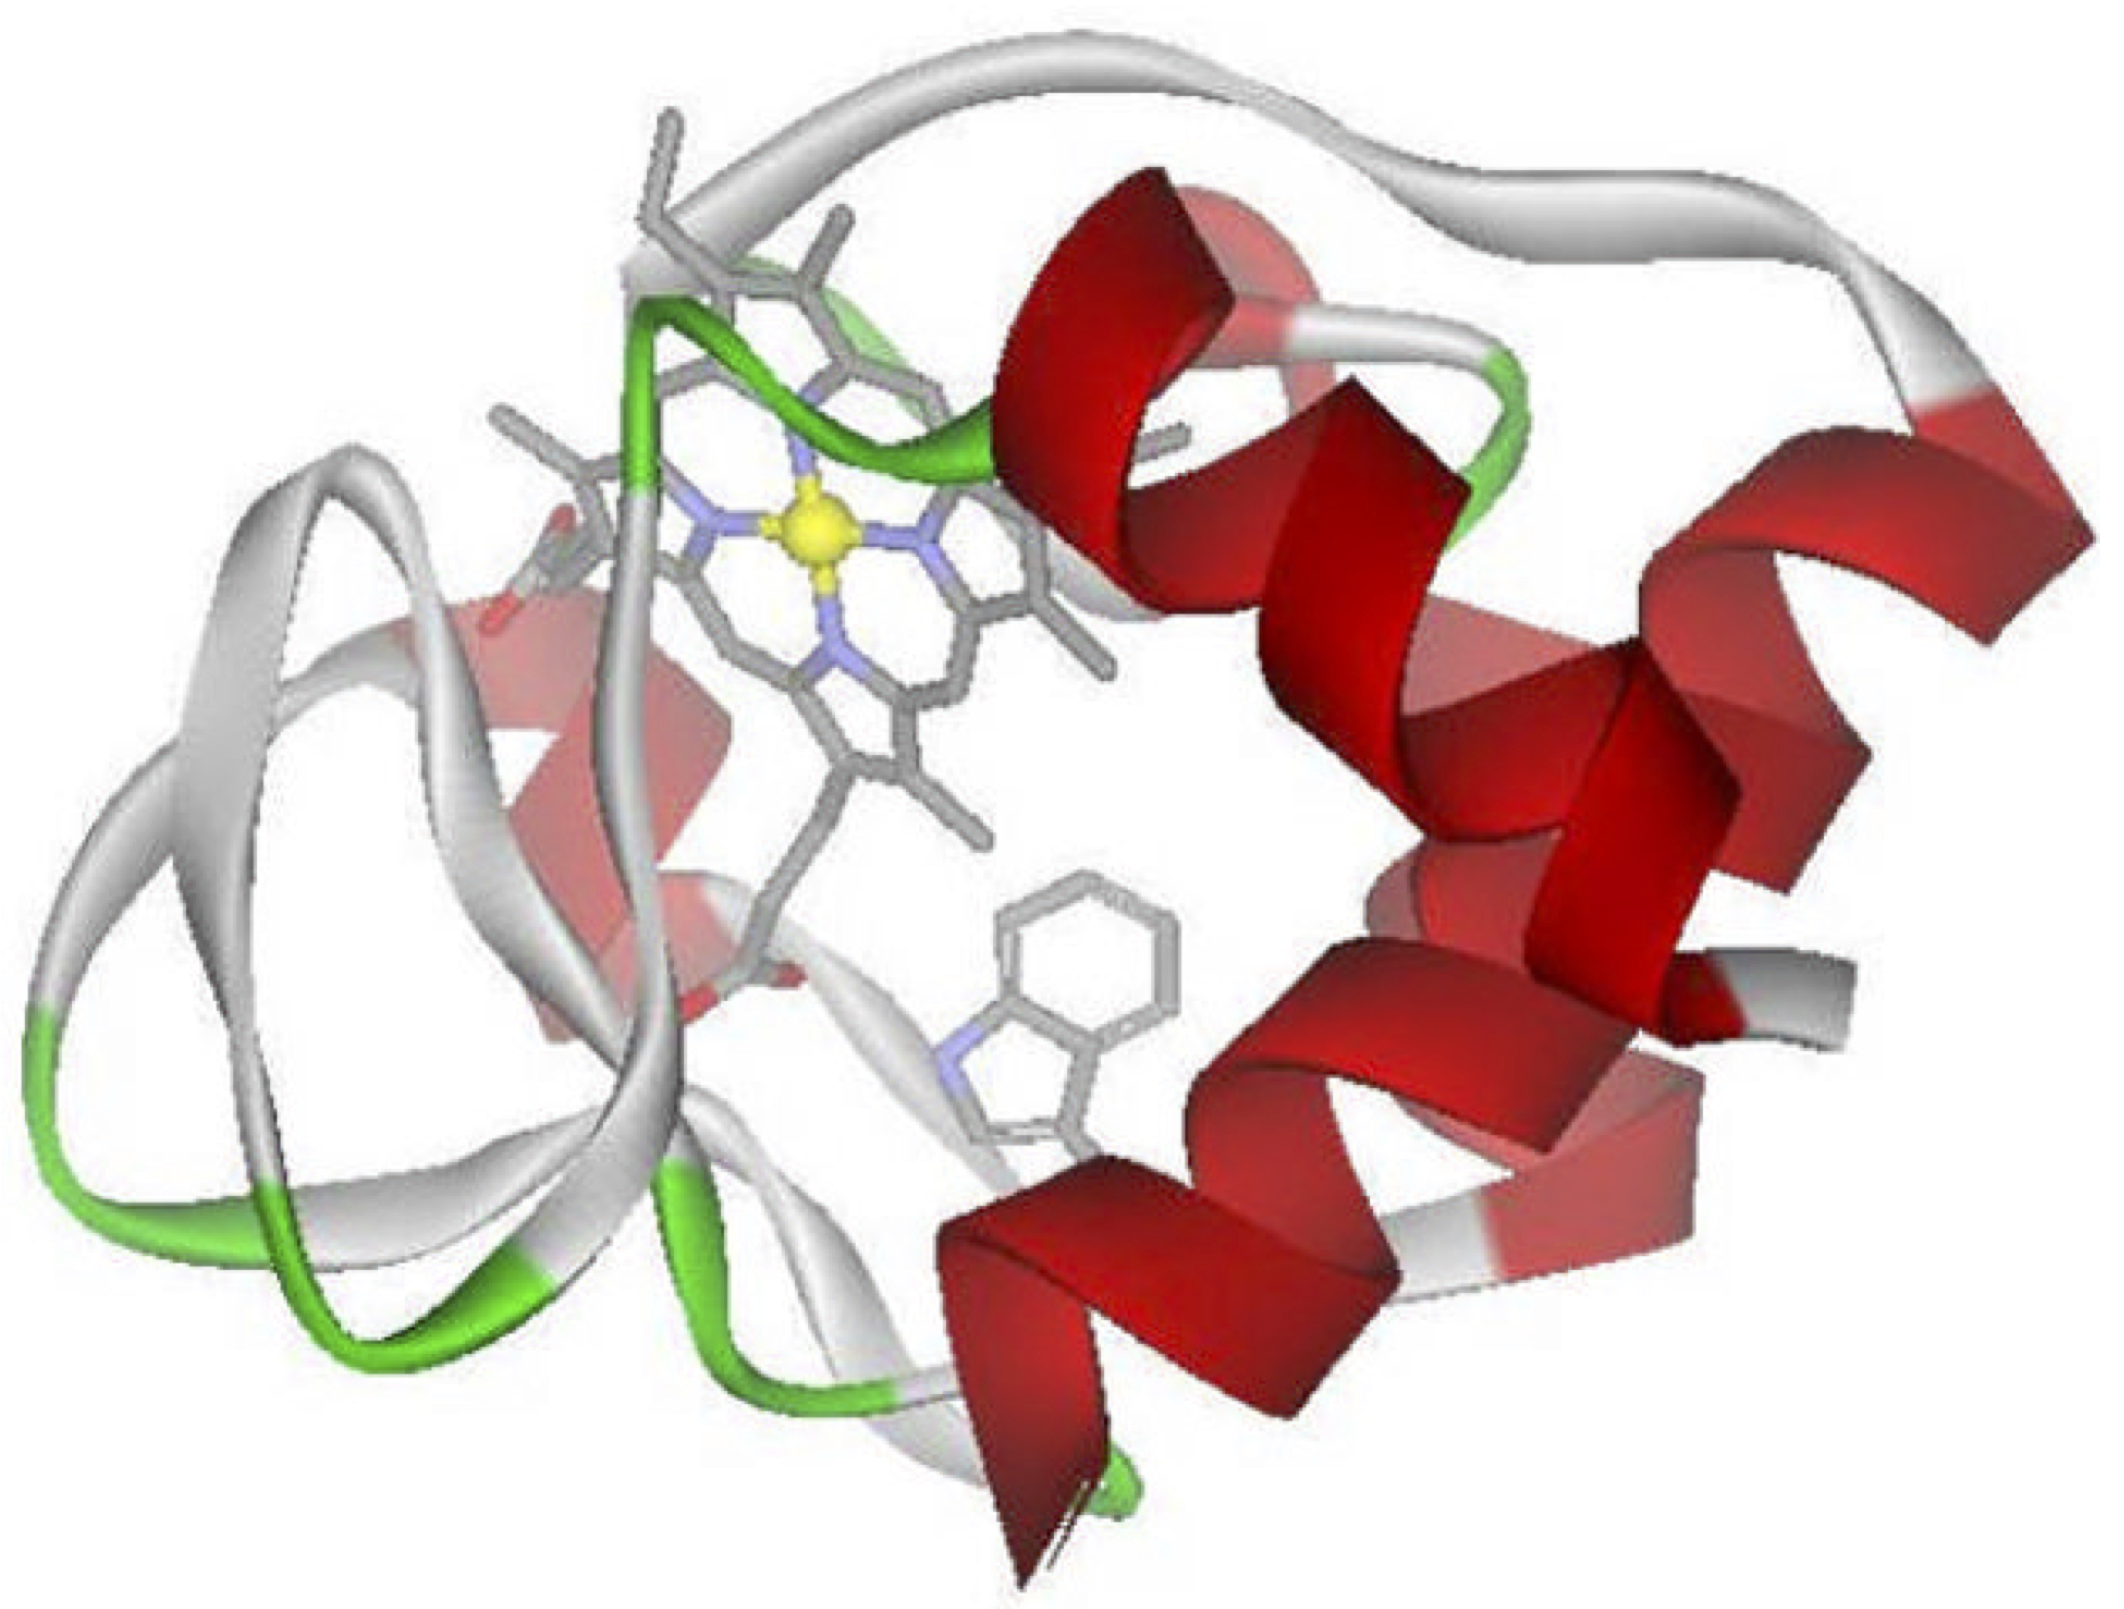
\includegraphics[width=.9\textwidth]{../images/cyt_c.png}
	\caption{Crystal structure of cyt \emph{c} (\href{http://doi.org/10.2210/pdb1HRC/pdb}{PDB: 1HRC}). 
	Trp-59 and the heme group are shown.
	Image reproduced from \textcite{sanchez08}.
	}
	\label{fig:cyt_c}
\end{marginfigure}


% section intro (end)

\section{Theory} % (fold)
\label{sec:theory}

\subsection{Förster Resonance Energy Transfer} % (fold)
\label{sub:forster_resonance_energy_transfer}

According to Förster’s theory on energy transfer, the rate of energy transfer \( k_\mtext{T} \) is related to the lifetime of the donor in the absence of acceptor (\( \tau_\mtext{D} \)) and the distance between the donor and acceptor (\( r \)) via
\begin{equation}
	k_\mtext{T}\br{r} = \frac{1}{\tau_\mtext{D}} \br{\frac{R_0}{r}}^6 \, .
\end{equation}
The Förster distance, \( R_0 \), is the critical distance for energy transfer, and is defined as the distance at which the efficiency of energy transfer is \SI{50}{\percent}. 
Förster distances typically range from \SIrange{20}{60}{\angstrom}, and can be calculated using the relationship
\begin{equation}
	{R_0}^6 = \br{\SI{8.79e23}{\angstrom^6\Molar\per\cm\cubed}}
							\br{\kappa^2 n^{-4} \Phi_\mtext{D} J_\mtext{DA}} \, ,
  \label{eq:forster_dist}
\end{equation}
where \( \kappa^2 \) is the orientation factor between the transition dipoles of the donor and acceptor, \( n \) is the refractive index of the solvent, \( \Phi_\mtext{D} \) is the quantum yield of the donor in the absence of acceptor, and \( J_\mtext{DA} \) is the overlap integral of the donor emission spectrum and the acceptor absorption spectrum. 
The numerical prefactor depends on the units of the overlap integral, which can be calculated as follows:
\begin{equation}
	J_\mtext{DA} = \frac{\int F_\mtext{D}\br{\lambda}
											 \varepsilon_\mtext{A}\br{\lambda} 
											 \lambda^4 \dd\lambda}
											{\int F_\mtext{D}\br{\lambda}\dd\lambda} \, .
  \label{eq:overlap_int}
\end{equation}
Here, \( J_\mtext{DA} \) is in \si{\per\Molar\cmc}, \( \lambda \) is in units of \si{\cm}, \( F_\mtext{D}\br{\lambda} \) is the fluorescence of the donor in the absence of the acceptor, and \( \varepsilon_\mtext{A}\br{\lambda} \) is the extinction coefficient of the acceptor in units of \si{\per\Molar\per\cm} at wavelength \( \lambda \). The energy transfer efficiency, \( E \), is defined by the following relationship:
\begin{equation}
	E = \frac{{R_0}^6}{{R_0}^6 + r^6} \, .
	\label{eq:dist_efficiency}
\end{equation}
Efficiency can be experimentally determined using the fluorescence intensities of the donor with and without the acceptor in the form of
\begin{equation}
	E = 1 - \frac{F_\mtext{DA}\br{\lambda}}{F_\mtext{D}\br{\lambda}} \, ,
	\label{eq:spec_efficiency}
\end{equation}
where \( F_\mtext{DA}\br{\lambda} \) is the fluorescence intensity of the donor in the presence of the acceptor and \( F_\mtext{D}\br{\lambda} \) is the fluorescence intensity of the donor in the absence of the acceptor. 

% subsection forster_resonance_energy_transfer (end)

\subsection{Free Energy of Protein Unfolding} % (fold)
\label{sub:free_energy_of_protein_unfolding}

Native tertiary structures of biomolecules can be disrupted by a variety of methods, including changes in temperature and \pH, as well as addition of chemical denaturants. 
Two common chemical denaturants, guanidinium hydrochloride and urea, are used to disrupt native protein structures easily. 
The mechanisms by which these denaturants unfold proteins is an active area of research, and hypotheses regarding their modes of action involve direct solvation of peptide bonds and other hydrophobic regions as well as significant modification of solvent structures. 
By measuring the relative concentrations of folded and unfolded proteins as a function of denaturant concentration, one generates an unfolding curve which can be further analyzed to determine protein stability. 

Spectroscopic techniques are commonly used to determine relative concentrations of folded and unfolded proteins for a given denaturant concentration. 
A critical requirement is that the folded and unfolded species exhibit unique spectroscopic signatures. 
Typical optical methods that may distinguish between native and denatured structures include circular dichroism, UV-Vis absorption spectroscopy, and fluorescence spectroscopy. 
Shifts in absorption/emission maxima as well as changes in intensities often reflect changes in global and local protein structures. 
By utilizing these spectroscopic shifts to monitor changes in population, unfolding curves can be generated to yield free energies of unfolding in the absence of denaturant. 

The simplest model of protein folding/unfolding describes a two-state system of folded (\ch{F}) and unfolded (\ch{U}) species:
\begin{equation}
  \ch{F <=> U} 
\end{equation}
The equilibrium consant and free energy of unfolding are then given as 
\begin{align}
	K_\mtext{eq} &= \frac{\ch{[U]}}{\ch{[F]}} \qquad \mtext{and} \\
	{}\gibbs*[subscript-right=\ch{U}]{} &= -RT \ln{K_\mtext{eq}} = -RT \ln{\frac{\ch{[U]}}{\ch{[F]}}} \, ,
\end{align}
where \gibbs*[subscript-right=\ch{U}]{} is the free energy of unfolding in the presence of the denaturant. 
Here, we are interested in the free energy of unfolding in the absence of denturant. 
A theoretical treatment described by \textcite{pace86,jones97} approximates a linear perturbation of free energy as a function of denaturant concentration wherein extrapolation of this relationship to zero denaturant concentration gives rise to the free energy of unfolding in the absence of denaturant, \gibbs*[subscript-right=\ch{H2O}]{}:
\begin{equation}
	\gibbs*[subscript-right=\ch{U}]{} = \gibbs*[subscript-right=\ch{H2O}]{} - m C \, ,
\end{equation}
where \( m \) reflects the rate of change of the Gibbs energy with respect to denaturant concentration and \( C \) is the molar concentration of denaturant. 
The denaturant concentration that gives rise to equal populations of folded and unfolded proteins is referred to as the midpoint concentration, \( C_\mtext{m} \). 

Here, \( m \) (\si{\kilo\cal\per\Molar\per\mole}) describes the rate of change of the free energy of denaturant with respect to denaturant concentration and \( C \) (\si{\Molar}) is the molar concentration of denaturant.  

The denaturant concentration that gives rise to equal populations of folded and unfolded proteins is referred to as the midpoint concentration, \( C_\mtext{m} \).  At \( C_\mtext{m} \), the free energy of unfolding is zero so that
\begin{equation}
	\gibbs*[subscript-right=\ch{H2O}]{} = m C_\mtext{m} \, .
	\label{eq:gibbs_h2o}
\end{equation}

Using the definition of fraction of unfolded molecules, \( f \), given by:
\begin{equation}
	f = \frac{\ch{[U]}}{\ch{[U]} + \ch{[F]}} \, ,
	\label{eq:conc_frac}
\end{equation}
it is relatively straighforward to obtain the following equation:
\begin{equation}
	f = \frac{ \exp\br{ -m \br{\frac{C_\mtext{m} - C}{RT}}}}{1 + \exp\br{-m \br{\frac{C_\mtext{m} - C}{RT}}}} \, .
	\label{eq:fold_frac}
\end{equation}
Experimental data points in an unfolding curve are fit to \cref{eq:fold_frac}, with \( f \) and \( C \) as dependent and independed variables, respectively, to yield values for \( m \) and \( C_\mtext{m} \). 
Knowledge of the variables \( m \) and \( C_\mtext{m} \) then allows for determination of the Gibbs energy of unfolding in the absence of denaturant, \gibbs*[subscript-right=\ch{H2O}], using \cref{eq:gibbs_h2o}.

% subsection free_energy_of_protein_unfolding (end)

% section theory (end)

\section{Safety Precautions} % (fold)
\label{sec:safety_precautions}

\begin{itemize}
	\item Urea is a skin irritant, be sure to use gloves when handling urea and urea-containing solutions. If denaturant comes in contact with the skin, eyes, or respiratory tract, wash the affected area(s) with copious amounts of water. 
	\item Standard PPE should be worn at all times during the lab. 
	\item While cyt \emph{c} and phosphate buffer are relatively harmless, care should be taken while handling all proteins and buffers. Other proteins and buffers can be potentially hazardous. 
\end{itemize}

% section safety_precautions (end)

\section{Procedure} % (fold)
\label{sec:procedure}

In this experiment, you will determine the free energy of unfolding ferric cyt \emph{c} using the chemical denaturant urea. 
You will monitor changes in fluorescence from Trp-59 as a function of urea concentration to generate an unfolding curve for cyt \emph{c} (part A).  
In part B, you will determine the Förster distance of the Trp--heme pair using a tryptophan model compound, \iupac{\N-acetyl-tryptophanamide}, to approximate the donor in absence of acceptor (FD).  
The cyt \emph{c} absorption spectrum is used to determine \( \varepsilon_\mtext{A} \br{\lambda} \) of the acceptor. 
Finally, in the analysis, you will combine the knowledge gained in parts A and B to determine changes in distance between Trp-59 and the heme moiety as a function of denaturant. 

\subsection{Part A: Measurement of the Unfolding Curve} % (fold)
\label{sub:part_a_measurement_of_the_unfolding_curve}

\begin{enumerate}
	\item Turn on the instrumentation (fluorescence and absorption spectrometers) immediately upon arriving in the laboratory to allow the electronics to warm up and stabilize. 
	\item Prepare a stock solution (\SI{50}{\mL}) of \SI{20}{\milli\Molar} \pH{7.4} phosphate buffer. 
	This buffer is called \ch{KP_{\emph{i}}}. 
	Both components of the conjugate acid--base pair should be weighed out separately to obtain the desired ratio and then dissolved in water. 
	Use \iupac{potassium phosphate monobasic} (CAS 7778-77-0) and \iupac{potassium phosphate dibasic} (CAS 7758-11-4).
	\label{step:buffer_stock}
	\item Prepare a stock solution (\SI{50}{\mL}) of \SI{10.0}{\Molar} \iupac{urea} (CAS 75-13-6) in \SI{20}{\milli\Molar} \ch{KP_{\emph{i}}}. 
	You should add the \iupac{urea} and phosphates to an empty volumetric flask and add water up to the mark. 
	This solution is called urea/\ch{KP_{\emph{i}}}. 
	\label{step:urea_stock}
	\item Prepare a stock solution (\SI{0.8}{\mL} of \SI{\sim500}{\milli\Molar}) of cyt \emph{c} (CAS 9007-43-6) in \ch{KP_{\emph{i}}} (\( \varepsilon_{410} \) for cyt \emph{c} in this solution is \SI{\sim105000}{\per\Molar\per\cm}, \( \varepsilon_{530} \) is \SI{11200}{\per\Molar\per\cm}).
	\label{step:cyt_c_stock}
	\item Prepare several samples of \SI{\sim10}{\micro\Molar} cyt \emph{c} (\SI{1.5}{\mL} each) by mixing the appropriate amounts of stock solution from \cref{step:cyt_c_stock} with stock solutions made in \cref{step:buffer_stock,step:urea_stock} to achieve final urea concentrations of \SIrange{0.0}{10.0}{\Molar} in \SI{1.0}{\Molar} increments. 
	You should have \num{11} samples in \num{11} plastic Eppendorf tubes.
	\label{step:sample_prep}
	\item Record fluorescence and absorption spectra of \ch{KP_{\emph{i}}}, \iupac{urea}/\ch{KP_{\emph{i}}}, and each of the \num{11} samples prepared in \cref{step:sample_prep}. 
	The fluorescence spectra should be recorded with \( \lambda_\mtext{ex} \) set to \SI{290}{\nm} and \( \lambda_\mtext{det} \) should be scanned from \SIrange{350}{500}{\nm}. 
	Use ``high'' sensitivity and \SI{5}{\nm} slits for both excitation and emission. 
	These spectra will be used to determine the free energy of unfolding of cyt \emph{c} using fluorescence shanges of Trp-59 as the probe. 
	You will see a large peak at \SI{\sim323}{\nm} in the spectra of the buffers (\ch{KP_{\emph{i}}} and \iupac{urea}/\ch{KP_{\emph{i}}}) as well as in some of your cyt \emph{c} samples. 
	Discuss the origin of this peak with your lab instructor. 
	\label{step:fluor_spec}
\end{enumerate}

% subsection part_a_measurement_of_the_unfolding_curve (end)

\subsection{Part B: Determination of the Förster Distance} % (fold)
\label{sub:part_b_determination_of_the_forster_distance}

\begin{enumerate}
	\item Prepare \SI{5}{\mL} of a \SI{\sim10}{\micro\Molar} solution of the tryptophan model compound, \iupac{\N-acetyl-tryptophanamide} (NATA, CAS 2382-79-8) in \ch{KP_{\emph{i}}}. 
	The actual concentration is not important, as long as you are not saturating the fluorometer detector. 
	You may need to start with a concentrated stock solution of NATA and dilute it to the desired \SI{\sim10}{\micro\Molar}. 
	Regardless of how you prepare the sample, you must determine the actual concentration based on the value for the extinction coefficient at \SI{280}{\nm} (\( \varepsilon_{280} \) for NATA is \SI{5630}{\per\Molar\per\cm}).
	\label{step:nata_prep}
	\item Measure absorption and fluorescence spectra of the solution prepared in \cref{step:nata_prep}.
	\label{step:nata_spectrum} 
\end{enumerate}

% subsection part_b_determination_of_the_forster_distance (end)

% section procedure (end)
\section{Data Analysis} % (fold)
\label{sec:data_analysis}

\begin{enumerate}
	\item To obtain an unfolding curve, subtract the background fluorescence spectra of the buffer (\ch{KP_{\emph{i}}} or \iupac{urea}/\ch{KP_{\emph{i}}}) from the corresponding protein fluorescence spectra to obtain a corrected fluorescence spectrum. 
	These corrected spectra should be made using the following general procedure:
	\begin{description}
		\item [Spectrum A:] raw fluorescence from cyt \emph{c} in buffer/denaturant
		\item [Spectrum B:] raw fluorescence from buffer/denaturant
		\item [Corrected Spectrum:] Spectrum A \( - \) Spectrum B
	\end{description}
	The fluorescence intensity of the corrected spectrum at \SI{350}{\nm} should then be normalized for protein concentration (via the absorption value at \SI{530}{\nm}) and ploted as a function of \iupac{urea} concentration. 
	The \emph{y}-axis should be scaled from \numrange{0}{1}. 
	What is the free energy of unfolding?
	You will need \cref{eq:gibbs_h2o,eq:conc_frac}. 
	Fitting your data to \cref{eq:fold_frac} is best accomplished with advanced analytical software; the fitting routines in the SciPy library are well-suited to this task. 
	\label{step:spec_fit}
	\item If time permits, note the change in the absorption spectra as a function of denaturant concentration to generate an unfolding curve and determine the free energy of unfolding for cyt \emph{c}. 
	How do these results differ from \cref{step:spec_fit} and what are some possible origins of the differences (if any)?
	\item Use the fluorescence spectrum collected in \cref{step:nata_spectrum} along with the absorption spectrum of \SI{\sim10}{\micro\Molar} cyt \emph{c} (\SI{0.0}{\Molar} \iupac{urea}) from \cref{step:spec_fit} to calculate the Förster distance of the Trp--heme pair. 
	You will need \cref{eq:forster_dist,eq:overlap_int}.
	Determination of the integrated areas can be done numerically as a sum or using the integration functions built in to SciPy.\sidenote{Additional pertinent information for this system: 
	\begin{gather}
		\kappa^2 = 2/3 \, ,\\
		n = 1.4 \, ,\\
		\Phi_\mtext{D} = 0.13
	\end{gather}}
	\label{step:dist_calc}
	\item Using \cref{eq:dist_efficiency} and your calculated \( R_0 \) from \cref{step:dist_calc}, make a plot of energy transfer efficiency, \( E \), as a function of distance, \( r \), between donor and acceptor. 
	This is the theoretical distance dependence of energy transfer for the donor--acceptor pair. 
	\item Use \cref{eq:dist_efficiency,eq:spec_efficiency} and the corrected and (concentration) normalized spectra from \cref{step:fluor_spec} to determine the distance between Trp-59 and the heme group as a function of denaturant concentration. 
	For \( F_\mtext{D} \), use the fluorescence intensity of NATA at the same concentration as the cyt \emph{c} samples. 
	Compare the distance between Trp-59 and the heme group for the fully folded protein (\SI{0.0}{\Molar} \iupac{urea}) with distances obtained from the known crystal structure (\href{https://www.rcsb.org/structure/1hrc}{PDB: 1HRC}). 
	How do these compare?
	\item What assumptions are made to determine \gibbs*[subscript-right=\ch{H2O}]{} from part A and intramolecular distances from part C\@? 
	Do these assumptions conflict?
\end{enumerate}

% section data_analysis (end)

\section{Questions and Further Thoughts} % (fold)
\label{sec:questions_and_further_thoughts}

\begin{enumerate}
	\item 
\end{enumerate}

% section questions_and_further_thoughts (end)

\nocite{*}
\printbibliography[category=cited]% default title for `article` class: "References"

\DeclareFieldFormat{labelnumberwidth}{\textbullet}
\printbibliography[%
  title={Further Reading},%
  resetnumbers,%
  omitnumbers,%
	notcategory=cited,%
	]
	
